\documentclass{report}
\usepackage{hyperref}
% WARNING: THIS SHOULD BE MODIFIED DEPENDING ON THE LETTER/A4 SIZE
\oddsidemargin 0cm
\evensidemargin 0cm
\marginparsep 0cm
\marginparwidth 0cm
\parindent 0cm
\textwidth 16.5cm

\ifpdf
  \usepackage[pdftex]{graphicx}
\else
  \usepackage[dvips]{graphicx}
\fi

\begin{document}
% special variable used for calculating some widths.
\newlength{\tmplength}
\chapter{Unit ok{\_}image}
\section{Description}
This is @image tag test.\hfill\vspace*{1ex}



Note that for dvi, eps image will be chosen (for pdf and html, jpg):

\begin{figure}
  \ifpdf
    
\includegraphics{image_1.jpg}
  \else
    
\includegraphics{image_0.eps}
  \fi
\end{figure}


Note that using the same image for the 2nd time will cause the same image to be included in the output (i.e. in the output we have \textit{one} copy of ok{\_}image{\_}picture.jpg, not \textit{two}).

\begin{figure}
  \ifpdf
    
\includegraphics{image_1.jpg}
  \else
    
\includegraphics{image_0.eps}
  \fi
\end{figure}


Now note that pdf format will choose pdf version of the image:

\begin{figure}
  \ifpdf
    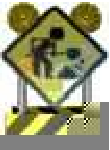
\includegraphics{image_2.pdf}
  \else
    
\includegraphics{image_0.eps}
  \fi
\end{figure}

\section{Constants}
\subsection*{Unimportant}
\begin{list}{}{
\settowidth{\tmplength}{\textbf{Description}}
\setlength{\itemindent}{0cm}
\setlength{\listparindent}{0cm}
\setlength{\leftmargin}{\evensidemargin}
\addtolength{\leftmargin}{\tmplength}
\settowidth{\labelsep}{X}
\addtolength{\leftmargin}{\labelsep}
\setlength{\labelwidth}{\tmplength}
}
\begin{flushleft}
\item[\textbf{Declaration}\hfill]
\begin{ttfamily}
Unimportant = 0;\end{ttfamily}


\end{flushleft}
\end{list}
\end{document}
